\documentclass[border=2mm,tikz]{standalone}
\usepackage{xcolor}
\definecolor{sRed}{HTML}{FF0033}
\definecolor{sBlue}{HTML}{0095D9}
\usetikzlibrary{calc, decorations.markings}

\tikzset
{%
    my arrow/.style={%
        decoration={%
            markings,
            mark=at position #1 with {\arrow{stealth}},
        },
        postaction={decorate}
    },
    pics/torus/.style={
        code={%
            \coordinate (-O) at (0, 0.75);
            \coordinate (-A) at ($(-O)+(195:1.75cm and 1cm)$);
            \coordinate (-B) at ($(-O)+(210:1.75cm and 1cm)$);
            \coordinate (-C) at ($(-O)+(330:1.75cm and 1cm)$);
            \coordinate (-D) at (250:3cm and 2cm);
            \coordinate (-G) at ($(-O)+(290:1.75cm and 1cm)$);
            \coordinate (-H) at (260:3cm and 2cm);
            \fill[gray!20] (-A) arc (195:210:1.75cm and 1cm)
                to [out=35,in=145] (-C)
                to [out=140,in=30] (-A);
            \fill[gray!20] (-D) arc (250:365:3cm and 2cm) to [out=250, in=10] cycle;
            \draw[thick, black] (0, 0) ellipse (3cm and 2cm);
            \draw[thick, black] (-B) to [out=35, in=145] (-C);
            % front curve
            \draw[thick, black] (-O) + (345:1.75cm and 1cm) arc (345:195:1.75cm and 1cm);
        }
    }
}

\begin{document}
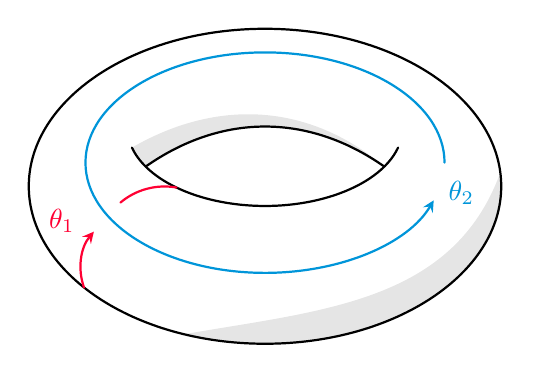
\begin{tikzpicture}[line cap=round]
    \pic (T) at (0, 0) {torus};
    \coordinate (-O) at (0, 0.75);
    \coordinate (-E) at ($(-O)+(230:1.75cm and 1cm)$);
    \coordinate (-F) at (220:3cm and 2cm);
    \coordinate (A1) at ($(0, 0.3) + (0:2.28cm and 1.4cm)$);
    \draw[sBlue, thick, -stealth] (A1) arc[start angle=0, end angle=340, x radius=2.28cm, y radius=1.4cm] node[xshift=0.35cm, yshift=0.1cm] {\(\theta_2\)};
    \draw[sRed, thick, -stealth] (-F) arc [start angle=200, end angle=140, radius=0.72cm] node[above, midway, xshift=-0.25cm, yshift=0.2cm] {\(\theta_1\)};
    \draw[sRed, thick] (-E) arc [start angle=80, end angle=130, radius=0.87cm];
\end{tikzpicture}
\end{document}
